\RequirePackage{plautopatch}
\documentclass[a4paper,11pt]{jsarticle}
\usepackage{color}
\usepackage{subcaption}
\usepackage{listings,jvlisting}
\usepackage{url}
% 数式
\usepackage{amsmath,amsfonts}
\usepackage{bm}
% 画像
\usepackage[dvipdfmx]{graphicx}
\lstset{
  stringstyle={	tfamily},
  commentstyle={	tfamily},
  basicstyle={	tfamily},
  columns=fixed,
  frame={tb},
  breaklines=true,
  columns=[l]{fullflexible},
  % numbers=left,%行数を表示したければonにする
  numberstyle={\scriptsize},
  xrightmargin=0em,
  xleftmargin=3em,
  stepnumber=1,
  numbersep=1em,
  tabsize=2,
  lineskip=-0.5ex,
  backgroundcolor=\color{white}
}
\usepackage{geometry}
\usepackage{tikz}
\geometry{left=25mm,right=25mm,top=20mm,bottom=20mm}
\begin{document}
\section*{1}
\begin{flalign*}
  (a) \#A &= 4 &&\\
  (b) \#B &= 47 &&\\
  (c) \#C &= 0 &&\\
  (e) \#E &= 6
\end{flalign*}

\section*{2.}
\begin{flalign*}
  \#U = 60 &&\\
  \#A = 25 &&\\
  \#N = 26 &&\\
  \#I = 26 &&\\
  \#(A \cap I) &= 9 &&\\
  \#(A \cap N) &= 11 &&\\
  \#(N \cap I) &= 8 &&\\
  \#(A^c\cap I^c\cap N^c) &= 8
\end{flalign*}

\section*{(a)}
\begin{flalign*}
  x &= \#(A\cap I\cap N) &&\\
  \#(A\cup I\cup N) &= 60 - 8 = 52 &&\\
  &= 25 + 26 + 26 - 9 - 11 - 8 + x  &&\\
  x &= 3
\end{flalign*}

\section*{(b)}
\begin{flalign*}
  \#(A  \cap I^c\cap N^c) &=  25 - (11+9-3) = 8  &&\\
  \#(A^c\cap I  \cap N^c) &=  26 - (8+9-3)  = 12 &&\\
  \#(A^c\cap I^c\cap N  ) &=  26 - (11+8-3) = 10 &&\\
\end{flalign*}

\section*{ベン図}
\begin{center}
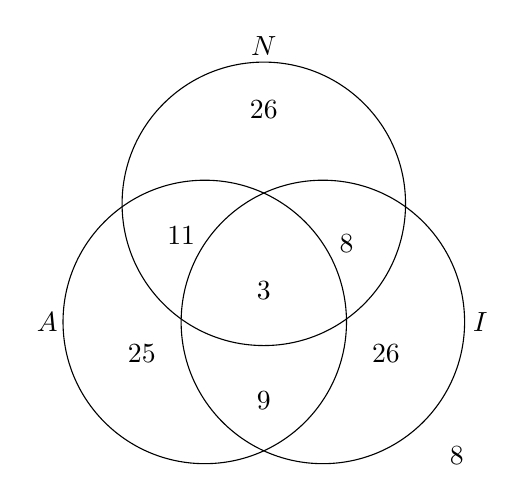
\begin{tikzpicture}
  \def\firstcircle{(0,0) circle (1.8cm)}
  \def\secondcircle{(1.5,0) circle (1.8cm)}
  \def\thirdcircle{(0.75,1.5) circle (1.8cm)}

  % Draw the circles
  \draw \firstcircle node at (-2,0) {$A$};
  \draw \secondcircle node at (3.5,0) {$I$};
  \draw \thirdcircle node at (0.75,3.5) {$N$};

  % Label regions
  \node at (-0.8,-0.4) {25};          % A only
  \node at (2.3,-0.4) {26};           % I only
  \node at (0.75,2.7) {26};           % N only
  \node at (0.75,-1) {9};              % A ∩ I only
  \node at (1.8,1) {8};              % I ∩ N only
  \node at (-0.3,1.1) {11};            % A ∩ N only
  \node at (0.75,0.4) {3};           % A ∩ I ∩ N
  \node at (3.2,-1.7) {8};           % Outside all sets

\end{tikzpicture}
\end{center}

\end{document}